\renewcommand{\imglabel}[1]{\put(2,5){\small\contour{black}{\textcolor{white}{\textbf{#1}}}}}
\begin{figure}[!ht]
	\centering
	\setlength{\resLen}{0.2\columnwidth}
	\addtolength{\tabcolsep}{-4pt}
	\begin{tabular}{cccc}
		Photo & Ours & [Aittala '06] & [Aittala '06]--Maps
		\\
		\begin{overpic}[width=\resLen]{bayesian/fig7/2_leather_4/target.jpg}
			\imglabel{Leather-4}
		\end{overpic} &
		\includegraphics[width=\resLen]{bayesian/fig7/2_leather_4/good1.jpg} &
		
\includegraphics[width=\resLen]{bayesian/fig9/2_leather_4/00.jpg} &
		\includegraphics[width=\resLen]{bayesian/fig9/2_leather_4/tex2x2.jpg}
		\\
		\begin{overpic}[width=\resLen]{bayesian/fig7/2_leather_6/target.jpg}
			\imglabel{Leather-6}
		\end{overpic} &
		\includegraphics[width=\resLen]{bayesian/fig7/2_leather_6/good1.jpg} &
		
\includegraphics[width=\resLen]{bayesian/fig9/2_leather_6/00.jpg} &
		\includegraphics[width=\resLen]{bayesian/fig9/2_leather_6/tex2x2.jpg}
		\\
		\begin{overpic}[width=\resLen]{bayesian/fig7/6_wood_4/target.jpg}
			\imglabel{Wood-4}
		\end{overpic} &
		\includegraphics[width=\resLen]{bayesian/fig7/6_wood_4/good1.jpg} &
		
\includegraphics[width=\resLen]{bayesian/fig9/6_wood_4/00.jpg} &
		\includegraphics[width=\resLen]{bayesian/fig9/6_wood_4/tex2x2.jpg}
		\\[-10pt]
	\end{tabular}
	\caption[Comparison with Aittala et al]{\label{fig:bayesian:aittala}
		\textbf{Comparison} with the Aittala et al.~\cite{aittala2016reflectance}.
		Results in the third column are rendered using tiled versions of texture maps shown in the fourth column.
		\\[0pt]
	}
\end{figure}
